\section{\textit{Tracking and Modifying Upper-body Human Motion Data with Dynamic Simulation}}

% ============================================================================
\subsection{Referência completa do artigo}

\begin{itemize}
  \item \textbf{Autores:} Victor B. Zordan, Jessica K. Hodgins
  \item \textbf{Local:} College of Computing and Graphics, Visualization and Usability Center, Georgia Institute of Technology
  \item \textbf{\textit{Journal}:} EUROGRAPHICS [Qualis A2]
  \item \textbf{Data:} Sept 1999
  \item \textbf{Referência:} \citeonline{bib:1999:upperbody}
\end{itemize}


% ============================================================================
\subsection{Resumo}

\subsubsection{Abstract}
Character animations produced with motion capture data have many of the stylistic details seen in human motion while those generated with simulation are physically realistic for the dynamic parameters of the character. We combine these two approaches by tracking and modifying human motion capture data using dynamic simulation and constraints. The tracking system generates motion that is appropriate for the graphical character while maintaining characteristics of the original human motion. The system imposes contact and task constraints to add dynamic impacts for interactions with the environment and to modify motions at the behavior level. The system is able to edit motion data to account for changes in the character and the environment as well as create smooth transitions between motion capture sequences. We demonstrate the power of combining these two approaches by tracking data for a variety of upper-body motions and by animating models with differing kinematic and dynamic parameters.

% ..........................................................
\subsubsection{Motivação}
A tecnica descrita no artigo indica uma maneira de combinar as tecnicas de captura de movimento e simulação dinamica para composição de animações que aparentam ser naturais e ao mesmo tempo respeitem as restrições físicas. Isso permite adaptar movimentos de captura para novas situações e fazer uma simulação reativa ao meio em que ela acontece e aos eventos que ocorrem.
% ..........................................................
\subsubsection{Propósito do artigo}
Simulação dinâmica garante uma animação fisicamente correta e se adapta naturalmente às mudanças de restrições do meio. Porém não é fácil simular os detalhes minunciosos da movimentação natural humana com um modelo simplificado do esqueleto e da musculatura.
A técnica de captura de movimento fornece um banco de dados com animações realistas e representam bem a naturalidade do movimento humano, ou de qualquer "ator" que tenha seu movimento capturado. Movimentos desse tipo são difíceis de se gerar proceduralmente, e por isso a técnica de captura ainda é a melhor para esse tipo de resultado.
% ..........................................................
\subsubsection{Técnicas utilizadas} 
\begin{itemize}
  \item Motion Capture
  \item Simulação Dinâmica
  \item Cinemática Inversa
  \item Cinemática Direta
  \item Controlador de trajetória
  \item Controlador de equilíbrio
\end{itemize}  

% ..........................................................
\subsubsection{Contribuição em relação a artigos anteriores} %mais ou menos 10 linhas
 \begin{itemize}
   \item Artigos anteriores tentaram combinar as técnicas mas utilizando abordagens diferentes. Neste artigo um modelo detalhado e completamente simulado foi utilizado no lugar de uma versão simplificada. Isso permite maior realismo na animação final.
   \item
 \end{itemize}  

% ============================================================================
\subsection{Metodologia}
% Descreva um pouco mais detalhadamente a metodologia e os resultados do artigo. 
% Inclua as figuras que achar mais relevantes.

\begin{figure}[ht]
  \centering
  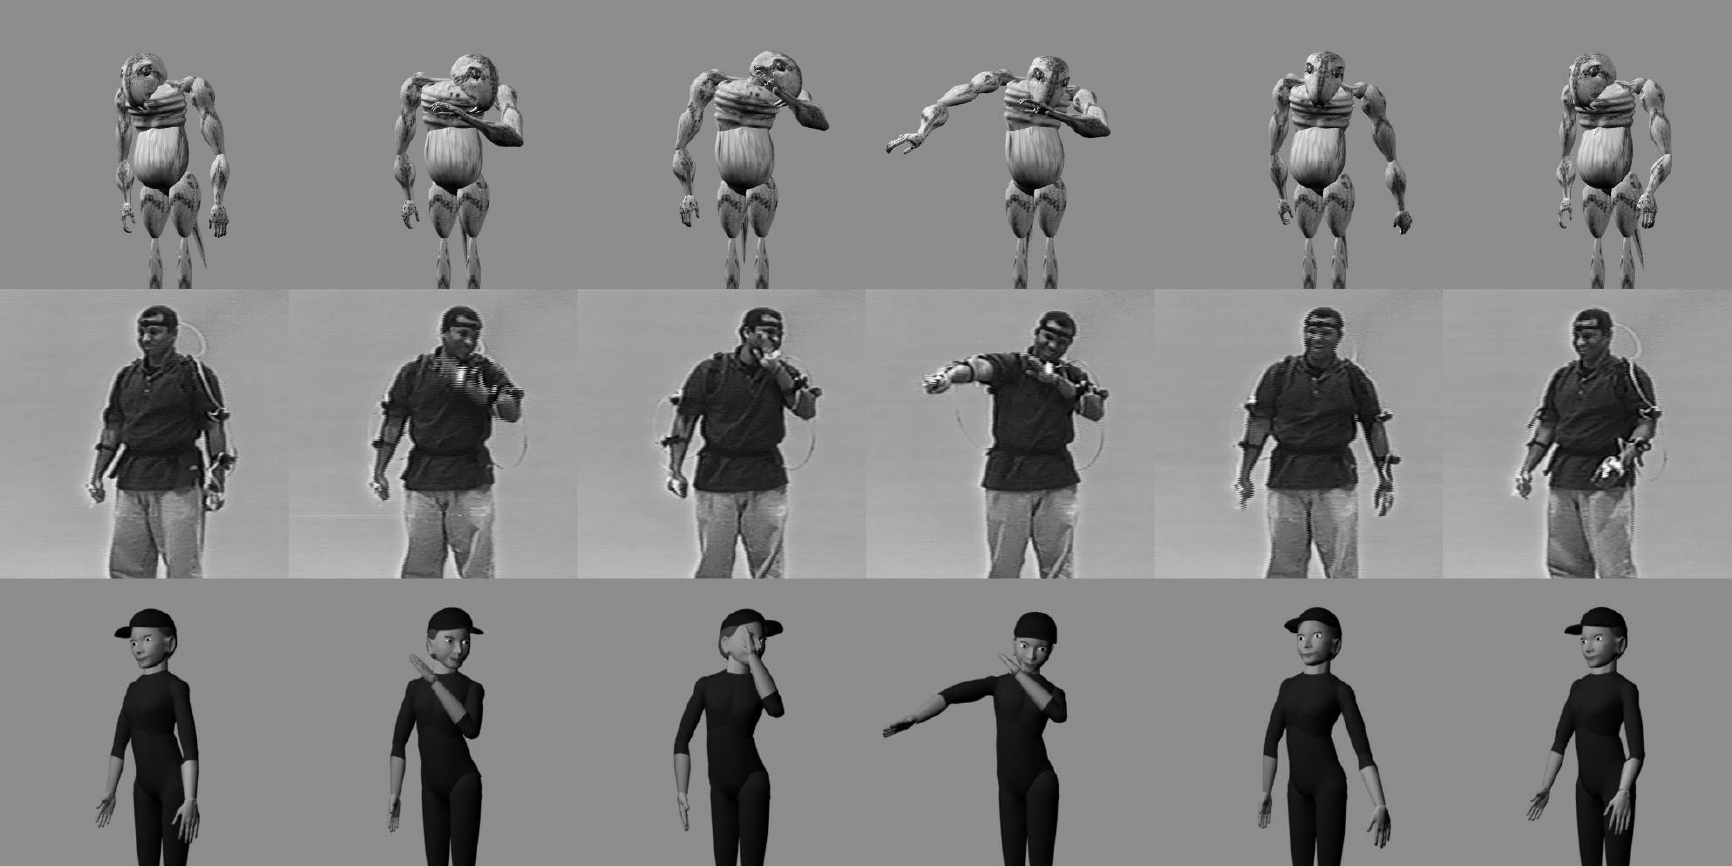
\includegraphics[height=150px]{artigos/1999_Tracking_and_Modifying_Upper-body_Human_Motion_Data_with_Dynamic_Simulation_zordan_TMU/fig_mocap.png}
  \caption{Captura de movimento mapeada em personagens virtuais.}
  \label{fig:1999:upperbody:fig1}
\end{figure}


\subsubsection{Motion Capture}

Existem diversas técnicas de motion capture, que tentam mapear movimentos reais para modelos virtuais. No artigo, eles utilizaram um ator com sensores de movimento no corpo. O resultado do mapeamento pode ser visto na figura \ref{fig:1999:upperbody:fig1}, onde no meio acompanhamos o processo de captura, e ao redor podemos ver o mesmo movimento mapeado em personagens com características físicas diferentes.

\begin{figure}[ht]
  \centering
  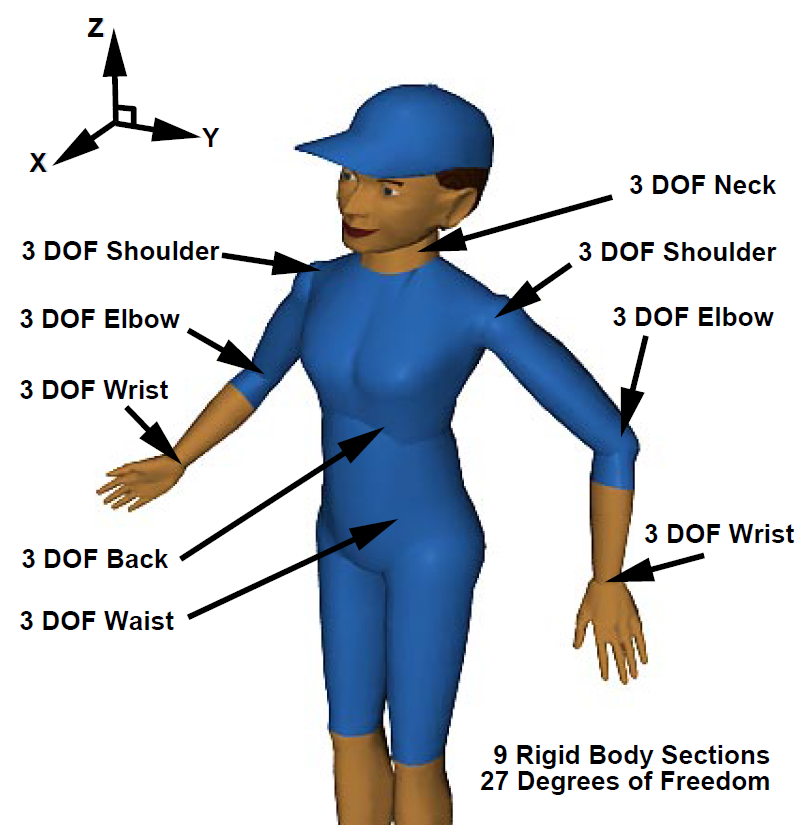
\includegraphics[height=150px]{artigos/1999_Tracking_and_Modifying_Upper-body_Human_Motion_Data_with_Dynamic_Simulation_zordan_TMU/fig_model.png}
  \caption{Este modelo tem 27 graus de liberdade controlados, com pernas estáticas. Outro modelo tem apenas 24 graus de liberdade, excluindo a articulação das costas. O modelo de corpo inteiro possui 48 graus de liberdade, com juntas adicionais nas pernas para manter o equilíbrio.}
  \label{fig:1999:upperbody:fig2}
\end{figure}

\subsubsection{Combinação das técnicas}

Para conseguir o resultado de combinar as duas ténicas, três adições são feitas ao sistema. Primeiramente, um gerenciador de colisões, para detectar interações com o ambiente. Segundo, controladores são adicionados. Esses controladores podem corrigir a movimentação do personagem diante das interações físicas, modificar a movimentação do personagem a nivel comportamental, adicionar noção de equilíbrio para manter o personagem de pé e animar graus de liberdade que não foram capturados previamente. Terceiro, os inputs de captura podem ser modificados e combinados para gerar novos movimentos, que juntamente com a simulação de física, se provaram suaves e realistas.

\begin{figure}[ht]
  \centering
  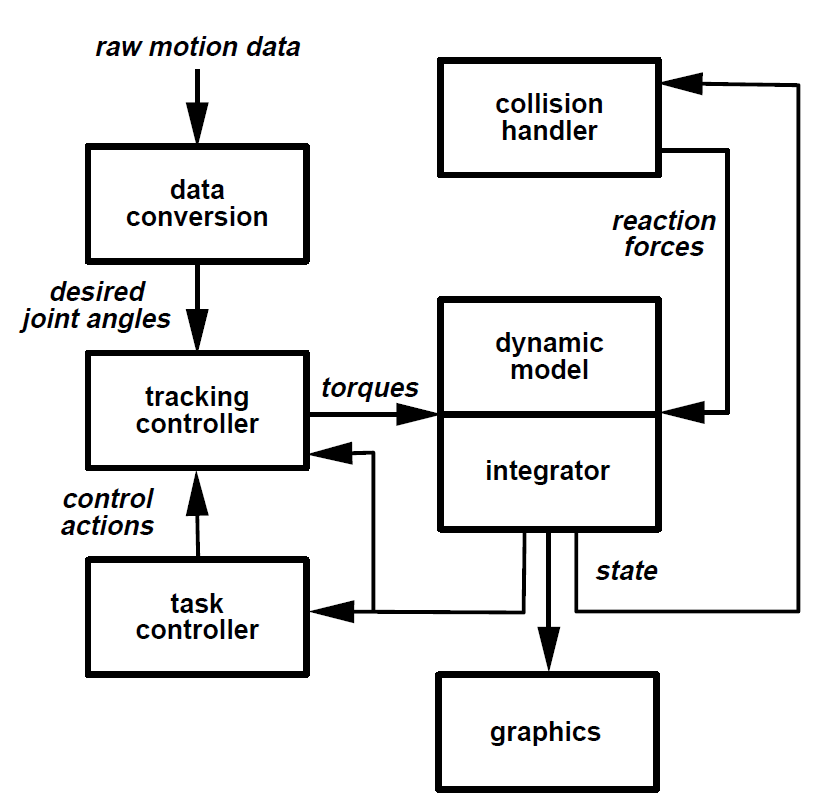
\includegraphics[height=150px]{artigos/1999_Tracking_and_Modifying_Upper-body_Human_Motion_Data_with_Dynamic_Simulation_zordan_TMU/fig_layout.png}
  \caption{O dado bruto de captura é convertido em angulos para as juntas, e são utilizados como valor a ser atingido pelos controladores de trajetória. Um controlador de tarefa e um gerenciador de colisão podem ser adicionados para gerar movimentos mais complexos e direcionar o comportamento.}
  \label{fig:1999:upperbody:fig3}
\end{figure}

\subsubsection{Simulação dinâmica e controle de trajetória}

Para que o modelo siga a animação capturada, um controlador de trajetória é utilizado. Ele aplica forças nas juntas de modo que o modelo tente acompanhar o movimento capturado. Porém, junto a este controlador, a simulação de física está presente para trazer as restrições do mundo para a simulação. Este caso é apropriado para gestos simples ou quando há uma correspondência boa entre o ator capturado e o personagem gráfico. O esquema pode ser visto na \ref{fig:1999:upperbody:fig3}.
A técnica citada é utilizada na parte superior do corpo. Para a parte inferior, o personagem pode ser mantido estático ou utilizar um controlador de equilíbrio para aumentar o realismo e manter o personagem de pé. A figura \ref{fig:1999:upperbody:fig2} mostra um exemplo de modelo que pode ser utilizado para a simulação, indicando os graus de liberdade de cada junta.
Para os cálculos, o modelo precisa ter valores de massa e momento de inércia. Para este trabalho, os valores foram estimados a partir dos modelos tridimensionais e valores supostos de densidade.
Por conta do custo elevado do cálculo de colisão, foram consideradas apenas colisões em partes do corpo que eram de se esperar que colidissem durante a simulação. Colisões entre partes do mesmo corpo foram desconsideradas.
O angulo e a posição de cada marcador é fornecida pelo sistema de captura, e assim é possivel calcular os angulos desejados em cada junta. O angulo é calculado pela fórmula:
\begin{equation}
  \label{eq:1999:upperbody:calc_angulo}
  \Theta_{desired} = \Theta_{ii}^T\Theta_{io}
\end{equation}
Onde $ \Theta_{ii} $ representa a matriz de transformação do objeto que aparece anteriormente na arvore hierárquica (objeto pai), e $ \Theta_{io} $ o objeto que aparece posteriormente (objeto filho). A raiz da árvore foi considerada na pélvis.
Para o cálculo do torque a ser aplicado em cada junta, a seguinte formula se aplica:
\begin{equation}
  \label{eq:1999:upperbody:calc_torque}
  \tau = k ( \theta_{desired} - \theta_{actual} ) - k_d ( \dot{\theta}_{actual} )
\end{equation}
onde $\theta_{actual}$ e $\theta_{desired}$ correspondem aos angulos atual e desejado da junta, e $\dot{\theta}_{actual}$ é a velocidade atual da junta. $k$ e $k_d$ são termos de ganho e amortecimento. O sistema funcionará como uma mola e um amortecedor, definindo um "músculo de primeira ordem".
Não são estabelecidos limites para as juntas pois considera-se que o movimento de captura respeita as restrições naturais do movimento.
O controlador então é ajustado para minimizar o erro $\epsilon$:
\begin{equation}
  \label{eq:1999:upperbody:calc_stiffness}
  \epsilon = \sum{||\theta_{desired}-\theta_{actual}||}
\end{equation}
Dessa forma o controlador irá gerar um movimento mais aproximado da captura de input.

\subsubsection{Restrições}

Restrições foram classificadas como restrições de ambiente, restrições de tarefas. Um exemplo de restrição dinâmica de ambiente poderia ser um personagem batendo em um tambor. O tambor faz parte da cena, e ao atingir, uma força impedirá a mão de atravessar o tambor, fazendo um movimento reativo realista. Uma restrição de tarefa seria por exemplo um personagem segurando um cajado, e tentando equilibrar o mesmo enquanto sacode no ar. Para isso, é colocado um controlador de tarefa na mão do personagem para dar um ar de realismo no movimento, como se ele realmente estivesse segurando o peso do cajado. Outro exemplo é o controlador usado nas pernas que tentam manter o personagem ereto enquanto executa as movimentações na parte superior do corpo, mantendo o centro de massa dentro da região dos pés.

\subsubsection{Modificando Inputs}
A ideia é modificar os dados de captura para gerar novos movimentos que não estavam inicialmente previstos, adaptando a novas situações. Uma possibilidade é o uso de cinemática inversa, como no caso das crianças batendo palmas. O movimento foi capturado a partir de um adulto, mas devido as diferentes proporções dos corpos, um novo offset para as mãos teve de ser definido. A solução retratada no artigo mantém a mão com a mesma orientação, mudando sua posição para a desejada, e então o sistema é resolvido. É possível utilizar cinematica inversa também para modificar a velocidade de um movimento, mantendo o realismo. Existe um limite em que o sistema pode parar de funcionar e detectar contatos. Nesse caso, aumentar a duração do offset pode ajudar a contornar um pouco este problema.
Além disso, é possível combinar diferentes animações capturadas, concatenando ou interpolando, e então usar a sequencia final na simulação. Este é um problema comum a respeito de captura de movimentos e existem diversas soluções para isso. Para o exemplo das palmas, foi utilizada uma posição chave, e fazer que cada movimento comece e termine nessa posição. Isso permite uma solução imediata da concatenação de movimentos pois uma transição é imediata. Uma solução mais geral permite que qualquer animação se encaixe em outra, independentemente da sua configuração inicial e final. Para isso é dada uma função de peso que varia com o tempo, permitindo que uma animação transicione para a outra suavemente. Isto é feito com a seguinte fórmula:
\begin{equation}
  \label{eq:1999:upperbody:calc_stiffness}
  \theta_r(t) = \theta_a(t)(1-\omega(t)) +   \theta_b(t)\omega(t), 0<=\omega(t)<=1, t_0 <= t <= t_1
\end{equation}
Isso é uma $slerp$ entre cada angulo $\theta_a$ e $\theta_b$ em um determinado tempo $t$. A função $\omega$ utilizada pode ser uma função senoide de $ease in/ease out$.
O movimento resultante, por ser uma combinação de dois movimentos reais, acaba se tornando um movimento realistico.
% ..........................................................
\subsubsection{Resultados}
Um sistema que utiliza o modelo dinamico para seguir e modificar dados de captura de movimento para a parte superior do corpo foi apresentada, junto com diversos exemplos que demonstram o poder da técnica. É dificil ter naturalidade e estilo como métricas, e isso torna uma avaliação crítica do trabalho algo complicado. Uma possivel métrica é a comparação entre movimentos gerados e movimentos capturados brutos de mesma natureza que tenham sido capturados. Foi observado que o movimento pode apresentar uma suavidade maior que o movimento capturado. Isso faz com que algumas tarefas se tornem impossíveis de alcançar. Para resolver o problema, foi utilizada cinemática inversa. 
Varias sugestões foram propostas em situações onde o sistema não funciona muito bem. E apesar da solução apresentada não resolver o problema geral da simulação com dados de captura de movimento, é um passo considerável em relação a tentativas anteriores de produzir esse tipo de animação.

% ============================================================================
\subsection{Pontos fortes} %no máximo três
\begin{itemize}
  \item Combina o melhor da captura de movimento e da simulação física
  \item Personagem completamente simulado, permite animações mais realistas que artigos anteriores.
  \item Simulação detalhada da parte superior do corpo, que é relevante por conta da expressividade dos braços e da cabeça humana.
\end{itemize}  

% ============================================================================
\subsection{Limitações} %no máximo três
\begin{itemize}
  \item Outros artigos permitem simulações mais complexas, como saltos e corridas, porém eles utilizam um modelo simplificado de simulação.
  \item É restrito à parte superior do corpo, sendo a simulação da parte de baixo apenas para manter o equilíbrio, ou uma animação fixa.
  \item Para alguns movimentos é necessário o uso de cinemática inversa para posicionar elementos do corpo em posições desejadas, tornando o processo automático de sintese da animação menos automático.
\end{itemize} 

% ============================================================================
\subsection{Avaliação}
%\textbf{(a) Avanço considerável (\textit{Breakthrough}).}
 \textbf{(b) Contribuição significativa.}
% \textbf{(c) Contribuição modesta.}
% \textbf{(d) Contribuição fraca.}
% \textbf{(e) Sem contribuição.}

O artigo diminui consideravelmente a quantidade de input necessário para gerar uma animação fisicamente realista a partir de dados de captura, além de permitir modelos mais complexos e animações mais expressivas da parte superior do corpo humano, que representa melhor essa expressividade do corpo.

% ============================================================================
\subsection{Problema em aberto}
 \begin{itemize}
   \item Expandir a solução para animações mais complexas e utilizando o corpo inteiro com o mesmo nível de complexidade.
   \item Extrair informação relevante sobre o movimento a partir do dado de captura para criar novos comportamentos.
 \end{itemize}  

% ============================================================================
\subsection{Aspecto obscuro}
 \begin{itemize}
   \item Não fica claro quando a cinemática inversa deve ser utilizada para gerar um movimento desejado. Ela parece ser essencial para alguns tipos de atividades desejadas.
   \item A métrica para avaliar a técnica utilizada pelo autor. Mesmo tendo dado algumas sugestões, parece algo bem subjetivo.
 \end{itemize}  